%%%%%%%%%%%%%%%%%%%%%%%%%%%%%%%%%%%%%%%%%%%%%%%%%%%%%%%%%%%%%%%%%%%%%%%%%%%%%%%%%%
%%																				%%
%% File name: 		swhwcom.tex													%%
%% Project name:	Hochleistungsantenne										%%
%% Type of work:	T3X00 project work											%%
%% Author:			Sarah Brückner, Maximilian Stiefel, Hannes Bohnengel		%%
%% Date:			01st June 2016		     									%%
%% University:		DHBW Ravensburg Campus Friedrichshafen						%%
%% Comments:		Created in gedit with tab width = 4							%%
%%																				%%
%%%%%%%%%%%%%%%%%%%%%%%%%%%%%%%%%%%%%%%%%%%%%%%%%%%%%%%%%%%%%%%%%%%%%%%%%%%%%%%%%%

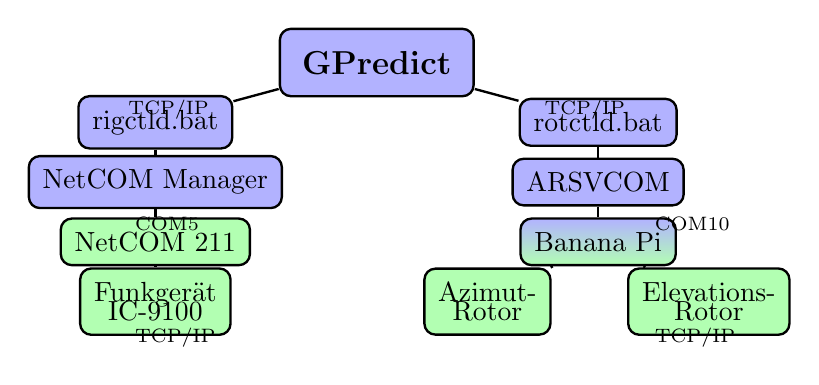
\begin{tikzpicture}[every node/.style = {shape=rectangle, rounded corners, draw, align=center, scale=1}, line width=0.3mm, level distance=1.8\baselineskip, level 1/.style = {sibling distance=16em}, level 2/.style = {sibling distance=8em}]
	\tikzstyle{top} = [fill=blue!30, inner sep=8pt, font=\bfseries\large]
	\tikzstyle{sw} = [fill=blue!30, inner sep=5pt]
	\tikzstyle{hw} = [fill=green!30, inner sep=5pt]
	\tikzstyle{hwsw} = [top color=blue!30, bottom color=green!30, inner sep=5pt]
	\tikzstyle{label} = [draw=none, font=\scriptsize, right]
	\node[top]{GPredict}
	child { node[sw]{rigctld.bat} 
		child { node[sw]{NetCOM Manager} 
				child { node[hw]{NetCOM 211}
					child { node[hw]{Funkgerät\\[-0.5em]IC-9100} } } } }
	child { node[sw]{rotctld.bat}
		child { node[sw]{ARSVCOM}
			child { node[hwsw]{Banana Pi} 
				child { node[hw]{Azimut-\\[-0.5em]Rotor} }
				child { node[hw]{Elevations-\\[-0.5em]Rotor} } } } };
	\node[label] at (2,-0.6) {TCP/IP};
	\node[label,left] at (-2,-0.6) {TCP/IP};
	\node[label] at (-3.2,-2.05) {COM5};
	\node[label] at (3.4,-2.05) {COM10};
	\node[label] at (-3.2,-3.5) {TCP/IP};
	\node[label] at (3.4,-3.5) {TCP/IP};
\end{tikzpicture}